\section{Introduction}
This document details the implementation of the thermal model software developed and divided into four main sections.  The first section explains how to install and report problems with the software. Section \ref{TM:sec:basic} explains the basic operation of the thermal software.  Section \ref{TM:sec:spread} presents an interface that links the thermal model with Microsoft Excel, allowing inputs to be easily modified.  Figure \ref{TM:fig:flow} contains a flow chart demonstrating how the various functions detailed in the first two sections (\ref{TM:sec:basic} and \ref{TM:sec:spread}) interact. Finally, in Section \ref{TM:sec:gui}, a complete graphical user interface is briefly presented that operates as a stand-alone Windows application.

A few notational conventions are utilized throughout this user manual:
\begin{itemize}
\item Monospaced typeface indicates a MATLAB m-file, function, or variable (e.g., \texttt{sobol.m}).
\item MATLAB code is provided in figure windows (e.g., Figure \ref{SA:fig:fang} when referenced many times).
\item MATLAB code is also presented in-line with the text as:
\begin{lstlisting}[style=inline]
>> 2+2
ans = 4 
>>
\end{lstlisting}\vspace*{0pt}
\end{itemize}

\begin{figure}[ht!]\centering
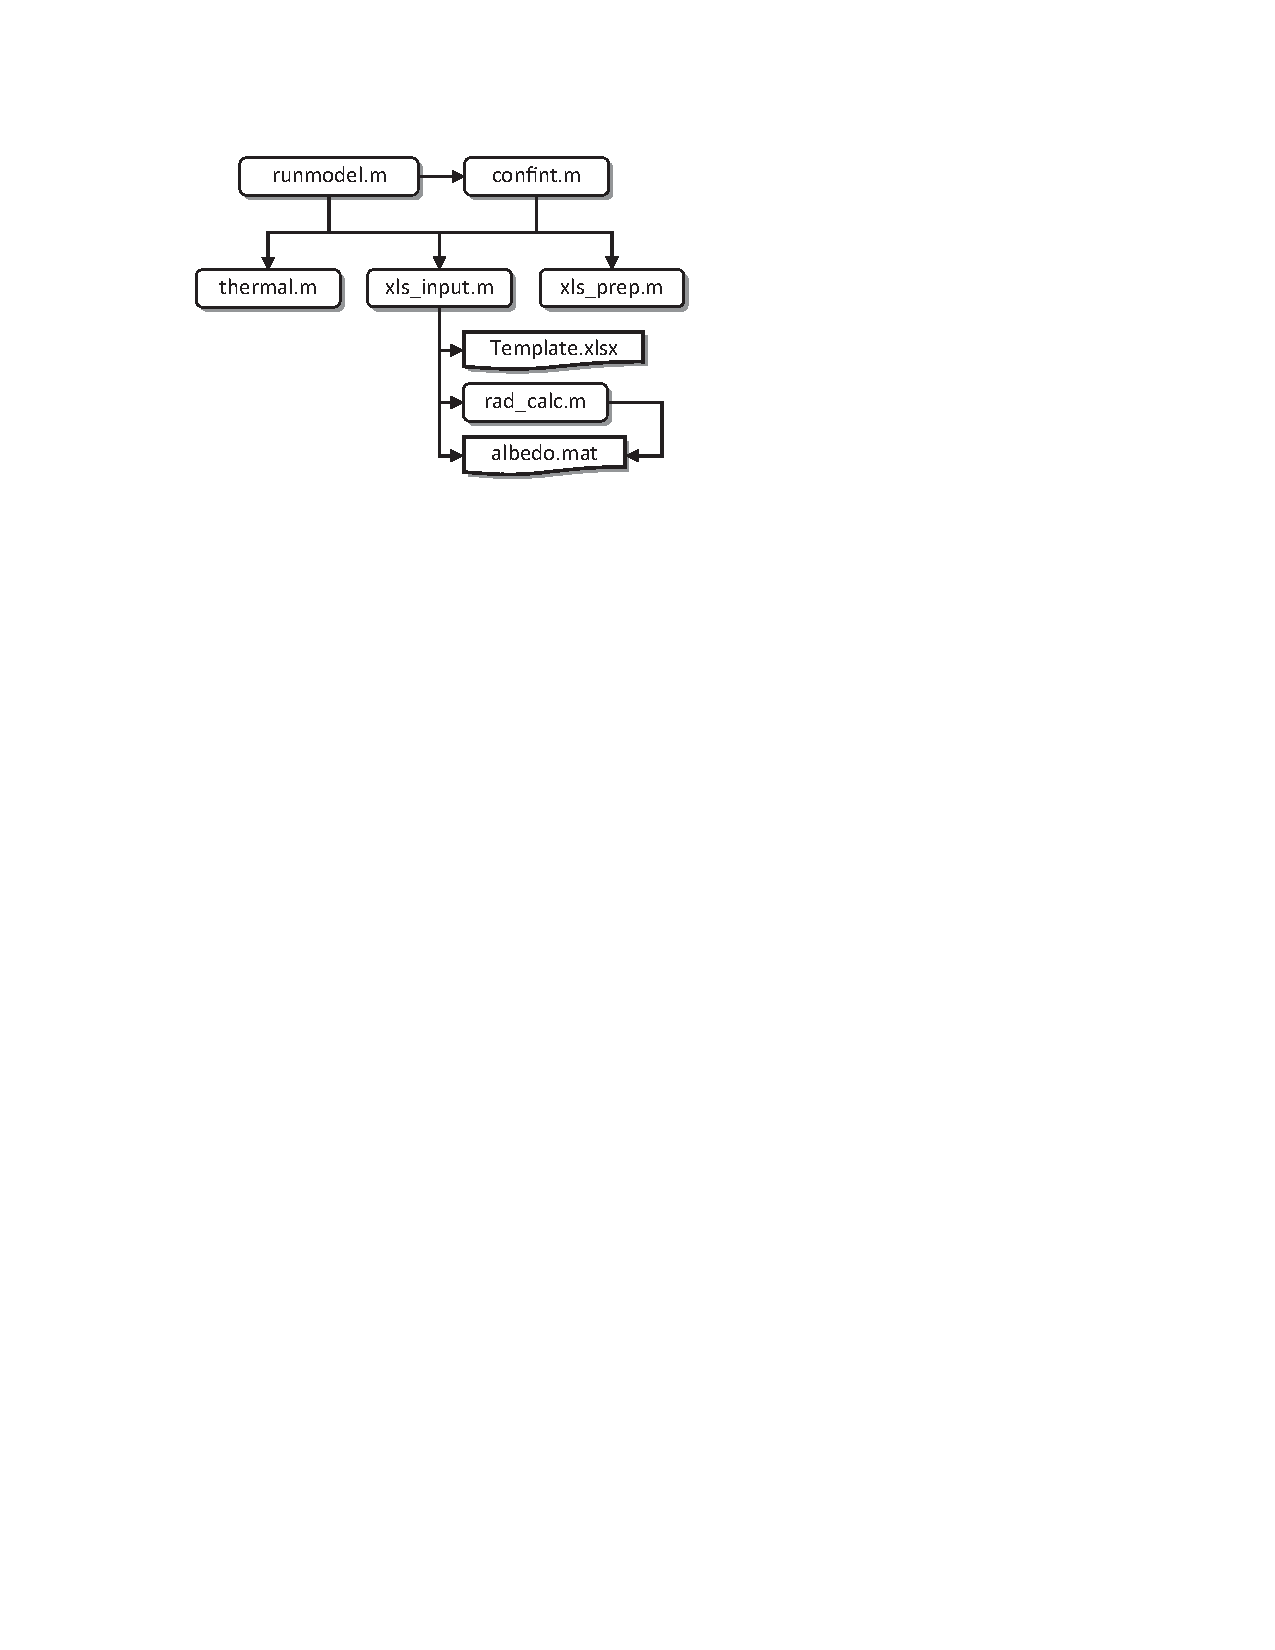
\includegraphics{figures/flow.pdf}
\caption{Flow chart demonstrating how the various functions discussed interact.}
\label{TM:fig:flow}
\end{figure}

\section{Installation and Bug Reporting}